\chapter{粒子から単純な量子場へ}

もう一度、単純な量子場を構築しよう。ただし、少し異なる角度からである。量子場理論への道は二つある。粒子から出発して、なぜ場が粒子にとって自然な言語なのかを発見する道と、波動場から出発して、なぜその励起が量子として現れるのかを発見する道である。どちらの道も有用である。ここでは最初の道にとどまる。

通常の量子力学は、一粒子、二粒子、あるいはその他の任意の固定された数を記述できる。自然はその制限を尊重しない。部屋の中の光子の数は、照明が放射を放出または吸収するたびに変化する。不安定な粒子は崩壊する。例えばベータ崩壊では、
\begin{equation}
n\longrightarrow p+e^-+\bar{\nu}_e,
\end{equation}
であるから、複数の粒子種の個数が同時に変化する。したがって我々は、あらゆる可能な占有数を含み、最終的にはそれらの間を移る過程をも含むのに十分大きな一つの量子力学を望む。

当面は大幅に単純化する。非相対論的な一つの粒子種がある。まずその状態空間を、任意の粒子数を保持できるように拡大し、その後になってから、より多くの粒子種、相対論、散乱、崩壊について論じる。数学はどれも特に難しいわけではないが、視点の変化は抽象的である。記法が考えを隠してしまわないように、十分ゆっくりと歩を進める価値がある。

\section{一粒子の出発点}

状態 \(|\psi\rangle\) にある一つの粒子から始める。その位置空間の波動関数は
\begin{equation}
\psi(x)=\langle x|\psi\rangle.
\label{eq:l07-wavefunction}
\end{equation}
である。この小文字の \(\psi\) は通常の複素数値関数である。それはまだ量子場ではなく、多粒子状態空間上の演算子でもない。

ボルンの規則によれば、
\begin{equation}
\rho_\psi(x)=|\psi(x)|^2=\psi^*(x)\psi(x)
\label{eq:l07-born-density}
\end{equation}
は粒子を \(x\) に見出す確率密度である。規格化された状態に対して、
\begin{equation}
\int dx\,\psi^*(x)\psi(x)=1.
\label{eq:l07-one-particle-normalization}
\end{equation}
である。右辺は全確率である。この問題にはちょうど一つの粒子しか含まれないので、それは粒子の数にもたまたま等しい。この一致は、ここでは自明であるが、後に有用な手がかりとなるであろう。

\begin{classroomqa}
\lecturetimestamp{00:09:13}
\audiencequestion{なぜ確率密度は \(\psi^*(x)\psi(x)\) の形をとらなければならないのか。}
\lecturerresponse{それは量子力学の公理の一つであるボルンの規則である。位置の結果 \(x\) に対する振幅は \(\langle x|\psi\rangle\) であり、確率密度はその絶対値の二乗である。それは後に用いる場の構成から導かれるものではない。}
\end{classroomqa}

\section{モード、直交性、完全性}

一粒子ヒルベルト空間には多くの有用な基底がある。位置固有状態は一つの基底をなす。任意のエルミート演算子の固有状態は、縮退と連続スペクトルに対する通常の但し書きとともに、別の基底をなす。エネルギーがまもなく重要になるので、一粒子エネルギー固有状態の完全正規直交系を選ぶ。
\begin{equation}
|1\rangle,\ |2\rangle,\ldots,
\qquad
\psi_i(x)=\langle x|i\rangle.
\end{equation}

箱の中の粒子は、添字 \(i\) を具体的なものにする。基底状態の波動関数は内部に節を持たず、次の状態は一つ持ち、より高い状態はより速く振動する。理想的な無限井戸に対して、それらは本質的に正弦波である。

\begin{figure}[htbp]
\centering
\includegraphics[width=0.94\linewidth]{lecture_07_frame_01.png}
\caption{講義板の上の箱のモード。左側の残りは一粒子ボルン密度と規格化であり、右側の井戸は \(\psi_1(x)\)、\(\psi_2(x)\)、および一般ラベル \(\psi_i(x)\) を示す。}
\lectureframe{00:08:25}
\end{figure}

同じモード構造を、ライブ板の遮蔽から分離することができる。
\begin{figure}[htbp]
\centering
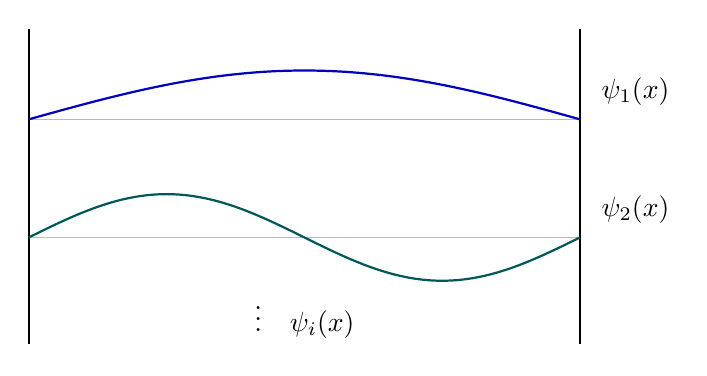
\begin{tikzpicture}[x=1cm,y=1cm]
  \draw[thick] (0,0) -- (0,4.0);
  \draw[thick] (7,0) -- (7,4.0);
  \draw[gray!55] (0,2.85) -- (7,2.85);
  \draw[gray!55] (0,1.35) -- (7,1.35);
  \draw[blue!75!black,thick,domain=0:7,samples=120]
    plot (\x,{2.85+0.62*sin(180*\x/7)});
  \draw[teal!70!black,thick,domain=0:7,samples=120]
    plot (\x,{1.35+0.55*sin(360*\x/7)});
  \node[right] at (7.15,3.20) {$\psi_1(x)$};
  \node[right] at (7.15,1.70) {$\psi_2(x)$};
  \node at (3.5,0.38) {$\vdots\quad\psi_i(x)$};
\end{tikzpicture}
\caption{定性的な箱のスケッチの清書。縦方向のずれは、表示のために二つの波動関数を分けているだけである。}
\end{figure}

正規直交性は
\begin{equation}
\int dx\,\psi_i^*(x)\psi_j(x)=\delta_{ij}.
\label{eq:l07-orthonormality}
\end{equation}
である。\(i=j\) ならば、状態は規格化されており、積分は 1 である。\(i\ne j\) ならば、二つの状態は直交しており、積分は消える。

完全性は、同じく重要な命題
\begin{equation}
\sum_i |i\rangle\langle i|=\mathbf 1.
\label{eq:l07-resolution}
\end{equation}
である。各 \(|i\rangle\langle i|\) は一つの基底方向への射影であり、完全基底にわたる和は恒等演算子である。任意のベクトルに作用させることは、そのベクトルを成分に分解し、再び組み立てるだけである。

ここで式~\eqref{eq:l07-resolution}を二つの位置状態ではさむ。
\begin{align}
\langle y|x\rangle
&=\sum_i\langle y|i\rangle\langle i|x\rangle \\
&=\sum_i\psi_i(y)\psi_i^*(x) \\
&=\delta(y-x).
\label{eq:l07-position-completeness}
\end{align}
星印は、ブラケットの順序が \(\langle i|x\rangle\) である因子に付く。\(x\) と \(y\) を入れ替えると、複素共役ではあるが等価な形が得られる。したがって、任意の完全正規直交基底はデルタ関数の表現を与える。正弦、余弦、振動子波動関数、エネルギー固有関数はすべて同じ役割を果たす。

\begin{classroomqa}
\lecturetimestamp{00:13:43}
\audiencequestion{完全性の和における二番目の波動関数は複素共役を伴うべきか。}
\lecturerresponse{はい。順序 \(\langle y|i\rangle\langle i|x\rangle\) では、因子は \(\psi_i(y)\psi_i^*(x)\) である。ブラケットの順序を見えるように保つことで、星印を推測したり置き忘れたりすることを防げる。}
\end{classroomqa}

これが我々に必要な一粒子の数学である。ここで状態空間を変更する。

\section{より大きな状態空間としてのフォック空間}

多数の同種粒子に対しては、各一粒子モードに何個の粒子が入っているかを記録する基底が便利である：
\begin{equation}
|n_1,n_2,n_3,\ldots\rangle.
\label{eq:l07-fock-basis}
\end{equation}
整数\(n_i\)はモード\(i\)の占有数である。このケットは、凝った記法で書かれた一粒子状態ではない。それはゼロ粒子セクター、すべての一粒子状態、すべての二粒子状態、等々を含む、より大きなヒルベルト空間に属する。そのより大きな空間はフォック空間と呼ばれる。

占有数を変えるために、各モードに対して生成演算子と消滅演算子を導入する：
\begin{equation}
a_i^\dagger,\qquad a_i.
\end{equation}
第一のものはモード\(i\)に粒子を一つ加え、第二のものは粒子を一つ取り除く。この段階では、調和振動子の言葉は帳簿付けの道具である：文字通りの振動するばねが存在する必要はない。振動子代数は、占有数を上げ下げするのに必要な仕組みをまさに与えてくれる。

モード数演算子は
\begin{equation}
\begin{aligned}
N_i&=a_i^\dagger a_i,\\
N_i|n_1,\ldots,n_i,\ldots\rangle
&=n_i|n_1,\ldots,n_i,\ldots\rangle.
\end{aligned}
\end{equation}
真空は
\begin{equation}
|0\rangle\equiv|0,0,0,\ldots\rangle,
\qquad
a_i|0\rangle=0
\quad\text{for every }i.
\label{eq:l07-vacuum}
\end{equation}
したがってモード\(i\)の一粒子状態は
\begin{equation}
|i\rangle=a_i^\dagger|0\rangle.
\label{eq:l07-mode-created}
\end{equation}
同じ記号\(|i\rangle\)は今や、一粒子基底ベクトルとしても、フォック空間の一粒子セクターに埋め込まれたそのベクトルとしても読むことができる。埋め込みは式~\eqref{eq:l07-mode-created}である；周囲の文脈が、どちらの空間が議論されているかを教えてくれる。

\section{モードを場にまとめる}

消滅場と生成場を次で定義する：
\begin{equation}
\Psi(x)=\sum_i \psi_i(x)a_i,
\qquad
\Psi^\dagger(x)=\sum_i \psi_i^*(x)a_i^\dagger.
\label{eq:l07-field-expansion}
\end{equation}
大文字であることが重要である。小文字の関数\(\psi_i(x)\)は複素数である；大文字の\(\Psi(x)\)はフォック空間上の演算子である。各空間点\(x\)において、式~\eqref{eq:l07-field-expansion}はモード演算子の異なる線形結合を与える。これが位置の演算子値関数の意味である。

自由粒子に対しては、モード関数は平面波\(e^{ikx}\)であってよい。そのとき式~\eqref{eq:l07-field-expansion}はフーリエ展開であるが、そのフーリエ係数が数ではなく演算子である点が異なる。古い用語では、通常の複素数を\(c\)数、量子演算子を\(q\)数と呼ぶ。モード関数は\(c\)数であり、すべてと可換である；\(a_i\)と\(a_i^\dagger\)が演算子としての性格を担う。

\(\Psi\)も\(\Psi^\dagger\)もエルミートではない。それらの随伴は互いに他方である。二つの組み合わせ
\begin{equation}
\Psi+\Psi^\dagger,
\qquad
i(\Psi^\dagger-\Psi)
\label{eq:l07-hermitian-combinations}
\end{equation}
はエルミートであり、観測量を表すことができる。しかし今のところ、場は粒子を局所的に生成し、消滅させ、数える道具として最も有用である。

\begin{classroomqa}
\lecturetimestamp{00:21:05}
\audiencequestion{演算子が\(x\)に依存するとはどういう意味か。}
\lecturerresponse{それは、\(x\)の各値が異なる演算子を選び出すという意味である。空間依存性は通常のモード関数にあり、その結果得られる各線形結合は同じフォック空間に作用する。}
\end{classroomqa}

\section{生成場がすること}

定義は、それが何をするかを問うて初めて有用になる。一粒子セクターの位置固有状態から始め、完全性の分解を挿入する：
\begin{align}
|x\rangle
&=\sum_i |i\rangle\langle i|x\rangle \\
&=\sum_i a_i^\dagger|0\rangle\,\psi_i^*(x) \\
&=\Psi^\dagger(x)|0\rangle.
\label{eq:l07-local-creation}
\end{align}
したがって\(a_i^\dagger\)は確定したモード\(i\)に粒子を生成するのに対し、\(\Psi^\dagger(x)\)は\(x\)に局在した粒子を生成する。理想化された位置基底では、その局在は超関数的である；物理的な準備では狭い波束を用いるであろうが、代数的な意味は同じである。

\begin{classroomqa}
\lecturetimestamp{00:24:48}
\audiencequestion{\(\sum_i|i\rangle\langle i|\)は射影か。}
\lecturerresponse{各項は一つの基底状態への射影である。完全な和はそれ自身が恒等演算子であり、恒等演算子の分解と呼ばれる。それを挿入しても状態は変わらないが、選ばれた基底における状態の成分が露わになる。}
\end{classroomqa}

式~\eqref{eq:l07-local-creation}は場の最初の直接的な粒子解釈である。我々は抽象的な演算子に空間的ラベルを付けただけではない。その空間点に粒子を作る操作を構成したのである。

\begin{classroomqa}
\lecturetimestamp{00:28:20}
\audiencequestion{位置空間の生成場には星印を付けるべきか、それともダガーを付けるべきか。}
\lecturerresponse{演算子の随伴にはダガーを用いる。星印は通常の波動関数\(\psi_i(x)\)の複素共役を表す；ダガーは\(a_i^\dagger\)と\(\Psi^\dagger(x)\)に付けるべきである。}
\end{classroomqa}

\begin{classroomqa}
\lecturetimestamp{00:28:36}
\audiencequestion{モード展開において生成演算子を波動関数の前後に動かしてよいか。}
\lecturerresponse{よい。\(\psi_i(x)\)は\(c\)数であるから、すべての演算子と可換である。\(a_i\)と\(a_j^\dagger\)のような非可換演算子の順序を変えるときだけ注意が必要である。}
\end{classroomqa}

\section{確率密度から粒子密度へ}

ではここで場をいじってみよう。最初の自然な表式は
\begin{equation}
\int dx\,\Psi^\dagger(x)\Psi(x).
\end{equation}
である。これは一粒子の規格化積分のように見えるが、その因子は今や演算子である。順序を変えずにモード展開を代入すると、
\begin{align}
\int dx\,\Psi^\dagger(x)\Psi(x)
&=\int dx
\left(\sum_i a_i^\dagger\psi_i^*(x)\right)\\
&\qquad\times\left(\sum_j a_j\psi_j(x)\right) \\
&=\sum_{i,j}a_i^\dagger a_j
\int dx\,\psi_i^*(x)\psi_j(x) \\
&=\sum_{i,j}a_i^\dagger a_j\,\delta_{ij} \\
&=\sum_i a_i^\dagger a_i.
\label{eq:l07-number-derivation}
\end{align}
となる。したがって総数演算子は
\begin{equation}
N=\sum_i N_i
=\int dx\,\Psi^\dagger(x)\Psi(x).
\label{eq:l07-total-number}
\end{equation}
である。ここで議論している状態では、有限エネルギーの励起は、モードエネルギーが十分高くなると占有数が消えていくので、可能なモードのリストが無限であっても、この総数は通常有限である。

被積分関数は局所的な粒子密度演算子である：
\begin{equation}
n(x)=\Psi^\dagger(x)\Psi(x).
\label{eq:l07-density}
\end{equation}
厳密に言えば、数学的な点で密度を測定することはない。小さな領域\(R\)に対しては、
\begin{equation}
N_R=\int_R dx\,n(x),
\label{eq:l07-regional-number}
\end{equation}
すなわちその領域内の粒子数を測定する。他の量子可観測量と同様に、\(N_R\)は任意の状態で確定した値をもつ必要はない。繰り返しの準備は異なる結果をもたらしうる。

\begin{classroomqa}
\lecturetimestamp{00:36:27}
\audiencequestion{\(\Psi^\dagger(x)\Psi(x)\)は多粒子確率密度なのか。}
\lecturerresponse{その直接的な意味は粒子密度である。多粒子確率振幅は一般にすべての粒子座標に依存する。これに対して局所的な双線形は、その領域にわたって積分されるとき、小さな領域内の粒子を数える。}
\end{classroomqa}

\begin{classroomqa}
\lecturetimestamp{00:38:28}
\audiencequestion{演算子\(a_i\)と\(a_i^\dagger\)は状態ベクトルにのみ作用し、一粒子波動関数には作用しないのか。}
\lecturerresponse{そのとおりである。それらは\(|n_1,n_2,\ldots\rangle\)のようなフォック空間の状態に作用する。それらに掛かる一粒子モード関数は通常の数であり、これらの昇降演算子が作用する対象ではない。}
\end{classroomqa}

占有数ケットは基底をなすが、最も一般的な状態ではない。それらは重ね合わせられうる。同じ総数がモード間で異なる分配をされる重ね合わせも含まれる。光子のような中性の種については、異なる総粒子数の重ね合わせも可能である。式~\eqref{eq:l07-regional-number}の演算子は、そのようなあらゆる状態において同じ操作的意味を保つ。

\begin{classroomqa}
\lecturetimestamp{00:40:01}
\audiencequestion{粒子密度を総数で割ると、\(x\)に粒子を見出す確率密度になるのか。}
\lecturerresponse{固定された\(N\)で大占有数の設定では、\(N_R/N\)は相対頻度であり、通常は一粒子確率を非常によく追跡する。それは一つの測定結果を確率と同一視する演算子の恒等式ではない。測定される計数は変動し、独立粒子描像では典型的には\(\sqrt N\)程度の量であり、例外的な試行は、そのような試行が起こりにくいとしても、確率から大きく異なりうる。}
\end{classroomqa}

\begin{classroomqa}
\lecturetimestamp{00:42:25}
\audiencequestion{一電子状態と零電子状態の重ね合わせで電荷保存はどうなるのか。}
\lecturerresponse{それは固定された電荷の閉じたセクターに用いられる種類の重ね合わせではない。同じ総電荷をもつ異なる分配を重ね合わせることはできる。光子は電荷を運ばないので、異なる光子数セクターはそのような問題を引き起こさない。電子数と陽電子数も、正味の電荷が固定されたまま一緒に変化しうる。}
\end{classroomqa}

\section{独立粒子のエネルギー}

次の可観測量はエネルギーである。まず互いに相互作用しない粒子に限定する。これは希薄系ではしばしば良い近似である。光子も原理的には高次過程を通じて相互作用するが、通常の実験室の放射は独立粒子描像が優れて成り立つほど希薄である。

\(\omega_i\)をモード\(i\)における一粒子のエネルギーとし、\(\hbar=1\)とする。モードとは一つの一粒子状態を意味する。このとき全ハミルトニアンは
\begin{equation}
H=\sum_i\omega_i N_i
=\sum_i\omega_i a_i^\dagger a_i.
\label{eq:l07-mode-hamiltonian}
\end{equation}
である。各占有モードは、粒子一つにつきその一粒子エネルギーを一度寄与する。

\begin{classroomqa}
\lecturetimestamp{00:48:16}
\audiencequestion{\(\omega_i\)は位置の関数か。}
\lecturerresponse{いいえ。それはモード\(i\)に付随するエネルギー固有値である。関数\(\psi_i(x)\)は位置に依存し、\(\omega_i\)はどのエネルギー準位が選ばれたかに依存する。}
\end{classroomqa}

値\(\omega_i\)は一粒子の時間に依存しないシュレーディンガー方程式によって決まる。
\begin{equation}
h=-\frac{\nabla^2}{2m}+V(x).
\label{eq:l07-one-particle-h}
\end{equation}
と定義すると、
\begin{equation}
h\psi_i(x)=\omega_i\psi_i(x).
\label{eq:l07-schrodinger-eigenvalue}
\end{equation}
となる。一次元では運動量演算子は\(p=-i\partial_x\)であり、\(p^2/(2m)\)は\(-\partial_x^2/(2m)\)となる。三次元では三つの二階導関数が合わさって\(-\nabla^2/(2m)\)となる。

\begin{figure}[htbp]
\centering
\includegraphics[width=0.94\linewidth]{lecture_07_frame_02.png}
\caption{黒板での\(p^2/(2m)+V(x)\)から一粒子シュレーディンガー固有値方程式の微分形への移行。式~\eqref{eq:l07-schrodinger-eigenvalue}はその整理された再構成である。}
\lectureframe{00:54:10}
\end{figure}

任意の規格化された一粒子波動関数に対して、よく知られた期待値は
\begin{equation}
\langle h\rangle_\psi
=\int dx\,\psi^*(x)h\psi(x).
\label{eq:l07-one-particle-energy-expectation}
\end{equation}
である。多粒子の式は、小文字の波動関数を演算子値の場で置き換えることによって示唆される。これはまだ証明ではない。正しさを今から検証する推測である：
\begin{equation}
H=\int dx\,\Psi^\dagger(x)h\Psi(x).
\label{eq:l07-field-hamiltonian}
\end{equation}

\section{まず答えを書き、次にそれを証明する}

方程式~\eqref{eq:l07-field-expansion}を提案されたハミルトニアンに代入する：
\begin{align}
\int dx\,\Psi^\dagger h\Psi
&=\int dx
\left(\sum_i a_i^\dagger\psi_i^*(x)\right)
h\left(\sum_j a_j\psi_j(x)\right) \\
&=\sum_{i,j}a_i^\dagger a_j
\int dx\,\psi_i^*(x)h\psi_j(x).
\label{eq:l07-h-expanded}
\end{align}
微分演算子\(h\)は\(x\)に依存する波動関数\(\psi_j(x)\)に作用し、モード演算子\(a_j\)には作用しない。シュレーディンガー方程式により、
\begin{equation}
h\psi_j(x)=\omega_j\psi_j(x).
\end{equation}
したがって、
\begin{align}
\int dx\,\Psi^\dagger h\Psi
&=\sum_{i,j}a_i^\dagger a_j\omega_j
\int dx\,\psi_i^*(x)\psi_j(x) \\
&=\sum_{i,j}a_i^\dagger a_j\omega_j\delta_{ij} \\
&=\sum_j\omega_j a_j^\dagger a_j.
\label{eq:l07-h-proof}
\end{align}
これはまさに方程式~\eqref{eq:l07-mode-hamiltonian}である。局所場の表式と全粒子エネルギーの和は同じ演算子である。

\begin{figure}[htbp]
\centering
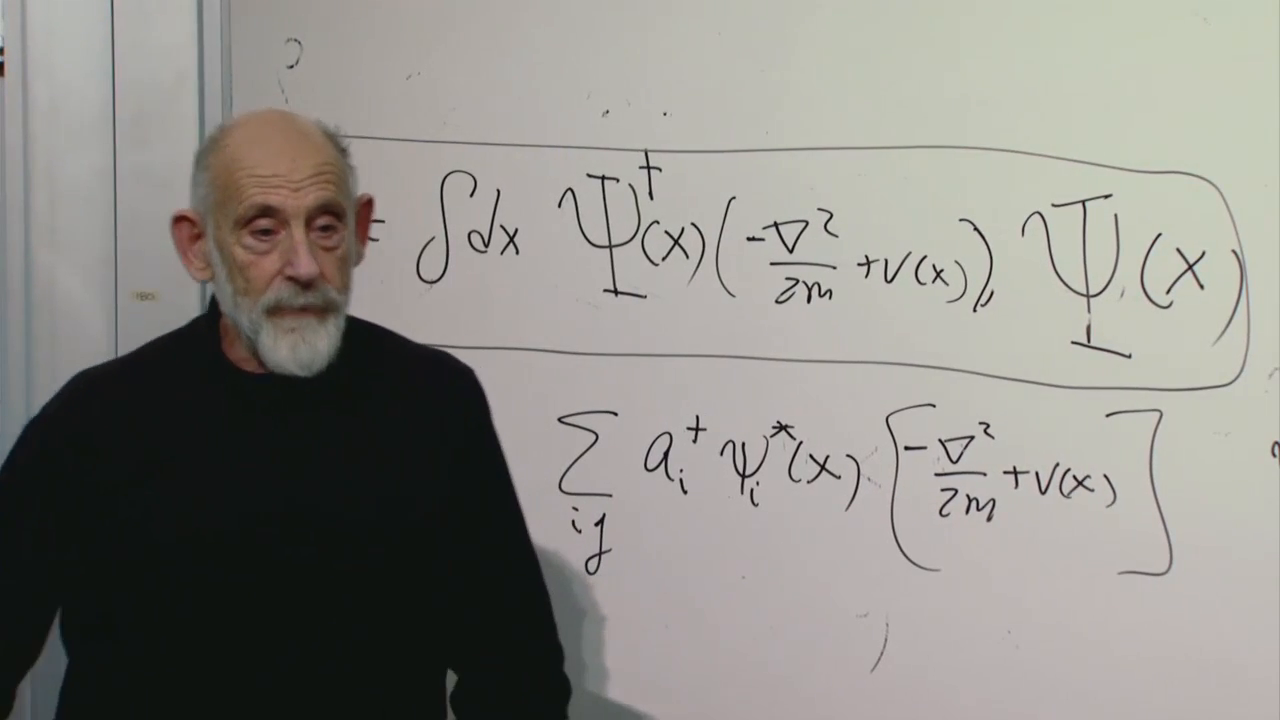
\includegraphics[width=0.94\linewidth]{lecture_07_frame_03.png}
\caption{黒板で強調された場のハミルトニアンと、その下に始まるモード展開による証明。ライブフレームは証拠として保持されている。方程式~\eqref{eq:l07-field-hamiltonian}--\eqref{eq:l07-h-proof}が完全な代数を復元する。}
\lectureframe{01:05:34}
\end{figure}

この導出では、生成演算子が消滅演算子と交換された箇所は一度もない。\(a_i^\dagger a_j\)の順序は最初から最後まで維持されている。自由に動かされた唯一の対象は\(c\)数波動関数とその固有値である。

\section{なぜこれが場なのか}

なぜ\(\Psi(x)\)を場と呼ぶのか。それは空間の各点で定義された演算子値の量であり、それから構成されるエルミート結合や双線形量は局所的可観測量だからである。密度\(n(x)\)と以下の局所エネルギー表式は二つの例である。この言葉の背後に隠れた追加の数学的判定基準はない。

この場は電磁場ではない。それは一粒子モードとハミルトニアン\(p^2/(2m)+V\)を与えた任意の非相対論的種、たとえばゆっくり運動する原子、中性子、陽子、電子を記述する。それらの粒子は対応する場の量子であり、光子が電磁場の量子であるのと同じ構造的な意味においてそうである。

\begin{classroomqa}
\lecturetimestamp{01:02:45}
\audiencequestion{多粒子系から上の式へ移る際、どこで場が入ってきたのか。}
\lecturerresponse{それは方程式~\eqref{eq:l07-field-expansion}で入ってきた：\(\Psi(x)\)は各空間点における演算子である。その後の導出は、その局所積が粒子密度とエネルギー密度を測ることを示している。位置依存性と演算子としての内容が、まさに構成されつつある場の構造である。}
\end{classroomqa}

\section{局所エネルギー密度}

方程式~\eqref{eq:l07-field-hamiltonian}は全エネルギーを空間上の積分として書く：
\begin{equation}
\begin{aligned}
H&=\int dx\,\mathcal H(x),\\
\mathcal H(x)
&=-\frac{1}{2m}\Psi^\dagger(x)\nabla^2\Psi(x)\\
&\quad+V(x)\Psi^\dagger(x)\Psi(x).
\end{aligned}
\label{eq:l07-hamiltonian-density}
\end{equation}
被積分関数はこのハミルトニアンに対する自然な局所エネルギー密度である。その局所形は一意ではない。たとえば部分積分により、運動項は
\begin{equation}
\mathcal H_{\rm kin}(x)
=\frac{1}{2m}\nabla\Psi^\dagger(x)\mathbin{\cdot}\nabla\Psi(x)
\label{eq:l07-kinetic-density}
\end{equation}
に境界項を除いて置き換えられる。通常の境界条件の下で、両方の表式は同じ全ハミルトニアンを与える。これが講義で言及された小さな曖昧さである。

\begin{classroomqa}
\lecturetimestamp{01:05:57}
\audiencequestion{エネルギー密度は全空間にわたって積分しなければならないのか。}
\lecturerresponse{全空間にわたる積分は全エネルギーを与える。より小さな領域にわたる積分は、その領域に割り当てられたエネルギーを与える。ただし、その全積分が同じハミルトニアンとなる局所密度を選ぶ際の通常の曖昧さが伴う。}
\end{classroomqa}

\begin{classroomqa}
\lecturetimestamp{01:06:25}
\audiencequestion{エネルギー式における大文字の\(N_i\)は小文字の\(n_i\)とどう異なるのか。}
\lecturerresponse{\(N_i=a_i^\dagger a_i\)は演算子である。整数\(n_i\)は占有数状態上でのその固有値の一つである。演算子は状態に作用し、その固有値は通常の数である。}
\end{classroomqa}

\begin{classroomqa}
\lecturetimestamp{01:06:46}
\audiencequestion{場のハミルトニアン自体をディラック記法でブラやケットとして書けるか。}
\lecturerresponse{いいえ。ブラとケットは状態ベクトルとその双対を表す。場とハミルトニアンはそれらの状態に作用する演算子である。\(\langle\Phi|H|\Phi\rangle\)のような期待値は両方の種類の対象を用いるのであり、それらを同一視してはならない。}
\end{classroomqa}

\section{一粒子の回復と古典場への接近}

拡大された形式は通常の一粒子量子力学を含んでいる。フォック空間を
\begin{equation}
N|\Phi\rangle=|\Phi\rangle.
\end{equation}
を満たす状態に制限する。その部分空間内では、場の構成はすべての一粒子状態とすべての一粒子予測を再現する。我々は古い理論を置き換えたのではなく、ゼロ個、二個、あるいは任意個の粒子も記述できる空間にそれを埋め込んだのである。

もう一方の極端では、非常に多数のボソンが占有するモードは、近似的に古典的な波のように振る舞うことができる。適切なコヒーレント状態または半古典状態では、期待値
\begin{equation}
\Phi_{\rm cl}(x,t)=\langle\Psi(x,t)\rangle
\end{equation}
は、自由非相対論的理論に対して、古典的に見える方程式
\begin{equation}
i\partial_t\Phi_{\rm cl}(x,t)
=\left(-\frac{\nabla^2}{2m}+V(x)\right)\Phi_{\rm cl}(x,t)
\label{eq:l07-classical-schrodinger}
\end{equation}
に従う。講義はこの関連を導出するのではなく述べるにとどめる。これは量子の集まりと波の場との間の橋渡しである。大きな占有数は相対的な揺らぎを抑え、適切な期待値を古典的に振る舞わせる。

したがって、この形式は簿記であると同時に物理でもある。それはすべての粒子数セクターを整理するが、干渉、エンタングルメント、そして量子粒子から古典的な波が現れることも捉えている。

\begin{classroomqa}
\lecturetimestamp{01:10:43}
\audiencequestion{なぜ生成演算子と消滅演算子は、積分の内部でまるで普通の数のように扱うことができるのか。}
\lecturerresponse{それらは互いに交換されたことは一度もない。通常のモード関数はそれらと可換であり、微分はそれらの関数にのみ作用する。消滅演算子を生成演算子の向こうへ動かすには交換子が必要となり、項が加わる可能性がある。証明の中ではそのような移動は一切行われていない。}
\end{classroomqa}

\section{ディラック記法の間奏}

混乱の一部は歴史的なものである。一粒子波動関数は波動方程式を満たし、一見すると古典場のように見えるが、同時に確率振幅でもある。初期の量子論はそれらの役割を分離し、次に電磁気学のような真に測定可能な波の場がどのように量子から作られるかを説明しなければならなかった。フォック空間と演算子値の場が、この見かけの矛盾を解決する。

ディラック記法はこの分離を極めて簡潔にする。ケットはベクトル空間に属し、ブラはその双対に属し、それらを並べると内積が形成される。分解
\begin{equation}
\sum_i|i\rangle\langle i|=\mathbf 1
\end{equation}
は、そのときほとんど自明になる。講義はこれを、数学者に量子力学を教えたときの逸話で例示する。数学的な内容はすでに馴染み深いものであったが、記法が日常的な操作をあまりに透明にしたため、構造が新しいものに見えたのである。要点は、ある分野に概念が欠けていたということではない。よく選ばれた記法は、許される操作を混同しにくくすることができるということである。

その教訓はここで重要である。今やいくつかの異なる演算子が存在する。
\begin{itemize}
\item \(h\) は一粒子波動関数に微分演算子として作用する。
\item \(a_i\) と \(a_i^\dagger\) はフォック空間の占有数状態に作用する。
\item \(\Psi(x)\)、\(\Psi^\dagger(x)\)、\(N\)、そして \(H\) もまたフォック空間に作用する。
\end{itemize}
式~\eqref{eq:l07-field-expansion}の展開は、最初の二つの設定を融合させることなく結びつける。

\begin{classroomqa}
\lecturetimestamp{01:18:16}
\audiencequestion{場は粒子の集まりを記述するための単なる形式なのか。}
\lecturerresponse{それらは形式であるが、空しいものではない。その局所的可観測量は測定可能であり、粒子は古典的な粒ではなく、干渉とエンタングルメントをもつ量子粒子である。場の演算子は、まさにそれらの測定可能な集団的性質を符号化している。}
\end{classroomqa}

\section{相対論的注意と電磁気学の余談}

これまでの構成は非相対論的である。相対論的物理学では運動量は依然として良い粒子ラベルであるが、鋭く局在した粒子の位置ははるかに微妙である。したがって、局所的な光子数密度は一般に、非相対論的な \(n(x)\) ほどきれいな対象ではない。エネルギー密度は依然としてよく定義され、より安全な局所的可観測量である。

講義は有用で、明示的にヒューリスティックな電磁気学的類推を与える。電場と磁場を複素ベクトル
\begin{equation}
\mathbf F=\mathbf E+i\mathbf B,
\qquad
\mathbf F^*=\mathbf E-i\mathbf B.
\label{eq:l07-riemann-silberstein}
\end{equation}
に組み合わせる。すると
\begin{equation}
\mathbf F^*\mathbin{\cdot}\mathbf F
=\mathbf E^2+\mathbf B^2,
\label{eq:l07-em-density}
\end{equation}
は、従来の単位で電磁エネルギー密度に比例する。これは文字通りには光子確率密度ではない。その大きさの二乗がエネルギー密度を測る、簡潔な場の変数と見るのがより良く、あるいは非公式には、光子エネルギーで重み付けられた光子密度と見ることもできる。

\begin{classroomqa}
\lecturetimestamp{01:19:10}
\audiencequestion{光子密度を電場の強さと同一視できるのか。}
\lecturerresponse{定性的に、そして注意深くならば可能である。相対論的光子では、局所的な粒子数は好ましい概念ではない。頑健な主張は、\(E^2+B^2\) がエネルギー密度に比例し、複素結合 \(\mathbf E+i\mathbf B\) がマクスウェル方程式をシュレーディンガー的な形にまとめるということである。}
\end{classroomqa}

\begin{classroomqa}
\lecturetimestamp{01:20:09}
\audiencequestion{相対論的な粒子は、なぜ位置は問題含みであるのに、確定した運動量をもつことができるのか。}
\lecturerresponse{運動量は相対論的な一粒子表現をきれいにラベルづけるが、厳密な局在は粒子の生成および相対論的な場の記述と衝突する。本講義ではその理論を展開しない。この警告は、現在の非相対論的な密度解釈の限界を示すものである。}
\end{classroomqa}

\section{順序と基底状態定数}

演算子の順序は気軽に変えてはならない。ボソンモードに対して、
\begin{equation}
a_i a_i^\dagger=a_i^\dagger a_i+1.
\end{equation}
したがって、正規順序 \(\Psi^\dagger h\Psi\) を逆順序 \((h\Psi)\Psi^\dagger\)、または適切に積分した対応物に置き換えると、交換子の寄与が加わる。モード基底では、これはモードあたり1量子のエネルギーの加法的な和である。これは基底状態すなわち零点の定数であり、連続体では正則化を要する。本講義ではこの問題をここで追及しない。ただ二つの順序が等しくないことを警告するのみである。

\begin{classroomqa}
\lecturetimestamp{01:22:04}
\audiencequestion{ハミルトニアンにおいて \(\Psi\) と \(\Psi^\dagger\) を入れ替えると何が起こるか。}
\lecturerresponse{それらの交換子を含めなければならない。したがって順序を逆にすると、同じ表式を再現するのではなく、状態に依存しない基底状態の寄与が加わる。表示されたハミルトニアンは正規順序 \(\Psi^\dagger h\Psi\) に保たれる。}
\end{classroomqa}

\section{最終テストとしての運動量}

最後の数分は、同じ昇格をもう一度繰り返す。一粒子に対して、
\begin{equation}
\langle p\rangle_\psi
=\int dx\,\psi^*(x)\left(-i\partial_x\right)\psi(x).
\label{eq:l07-one-particle-momentum}
\end{equation}
波動関数を場に置き換えると、全運動量演算子
\begin{equation}
P=\int dx\,\Psi^\dagger(x)\left(-i\partial_x\right)\Psi(x),
\label{eq:l07-field-momentum}
\end{equation}
が得られる。あるいは三次元では、
\begin{equation}
\mathbf P=\int d^3x\,\Psi^\dagger(\mathbf x)
\left(-i\boldsymbol\nabla\right)\Psi(\mathbf x).
\end{equation}
場は運動量を運ぶ。十分に強力なレーザーは壁に運動量を移して力を及ぼす。量子論的な記述では、その場の運動量は光子の運動量の和である。

式~\eqref{eq:l07-field-momentum} は演算子であり、期待値ではない。フォック空間の状態 \(|\Phi\rangle\) が与えられれば、次に
\begin{equation}
\langle P\rangle_\Phi=\langle\Phi|P|\Phi\rangle.
\end{equation}
を計算できる。期待値を形成するには演算子と状態の両方が必要である。可観測量とその平均を混同することは、本講義が確立しようと努めてきたまさにその区別を消し去ってしまうであろう。

\begin{classroomqa}
\lecturetimestamp{01:26:02}
\audiencequestion{表示された場の運動量はすでに平均運動量なのか。}
\lecturerresponse{いいえ。それは可観測量を表すエルミート演算子である。状態を与え、そのブラとケトの間に演算子を挟めば期待値が得られる。測定は依然としてその平均のまわりで揺らぎうる。}
\end{classroomqa}

ここが自然な区切りである。粒子から出発して、我々は局所的な生成・消滅場を構成し、それらを用いて粒子を数え、一粒子のエネルギーと運動量の和を場の演算子として書き換えた。次の段階は、もう一つの記法の変更ではない。場の演算子に物理的過程を表させることである。すなわち、粒子の崩壊、粒子の散乱、そして種の相互変換である。
